% ============ METADATA ============
\newcommand{\coursename}{CS202 - Programming Systems}
\newcommand{\reporttitle}{Super Mario OOP Project}

\documentclass[12pt]{article}
\usepackage{hcmus-report-template}

% ================== CUSTOM PACKAGES ==================
\usepackage{amsmath, amsfonts, float, graphicx, setspace}
\usepackage[colorlinks=true, linkcolor=blue, citecolor=red]{hyperref}
\usepackage{algorithm}
\usepackage{algpseudocode}
\usepackage{listings}
\usepackage{xcolor}
\usepackage{tabularx}
\usepackage{fancyhdr}

% ================== CODE STYLING ==================
\definecolor{codegreen}{rgb}{0,0.6,0}
\definecolor{codegray}{rgb}{0.5,0.5,0.5}
\definecolor{codepurple}{rgb}{0.58,0,0.82}
\definecolor{backcolour}{rgb}{0.95,0.95,0.92}

\lstdefinestyle{mystyle}{
    backgroundcolor=\color{backcolour},
    commentstyle=\color{codegreen},
    keywordstyle=\color{magenta},
    numberstyle=\tiny\color{codegray},
    stringstyle=\color{codepurple},
    basicstyle=\ttfamily\footnotesize,
    breaklines=true,
    breakatwhitespace=false,
    captionpos=b,
    keepspaces=true,
    numbers=left,
    numbersep=5pt,
    showspaces=false,
    showstringspaces=false,
    showtabs=false,
    tabsize=2
}
\lstset{
    style=mystyle,
    literate={:}{{\texttt{:}}}1
             {_}{{\texttt{\_}}}1
}
\vietnameselst  % Apply Vietnamese character support

% ================== HEADER & FOOTER ==================
\pagestyle{fancy}
\fancyhf{}
\fancyhead[L]{CS202 - Programming Systems}
\fancyhead[R]{HCMUS – Term 3}
\fancyfoot[R]{Page \thepage}
\setlength{\headheight}{29pt}
\renewcommand{\headrulewidth}{0.4pt}
\renewcommand{\footrulewidth}{0.4pt}

% ========== ENGLISH LABELS (deferred override) ==========
\AtBeginDocument{
  \renewcommand{\contentsname}{Table of Contents}
  \renewcommand{\listfigurename}{List of Figures}
  \renewcommand{\listtablename}{List of Tables}
  \renewcommand{\tablename}{Table}
}


% ================== DOCUMENT START ==================
\begin{document}
\raggedright  % <-- This makes main text left-aligned
\pagenumbering{roman}
\centering
\begin{center}

\includegraphics[width=0.2\textwidth]{img/hcmus-logo.png}
\end{center}

{\Large\bfseries TRƯỜNG ĐẠI HỌC KHOA HỌC TỰ NHIÊN \par}
{\Large\bfseries – ĐẠI HỌC QUỐC GIA THÀNH PHỐ HỒ CHÍ MINH \par}

\vspace{0.2cm}
{\large Khoa Công nghệ Thông tin \par}
\vspace{0.8cm}

{\Large\bfseries \coursename \par}
\vspace{1cm}
{\huge\bfseries \reporttitle \par}
\vspace{1.2cm}

{\Large Nhóm thực hiện: 11 \par}
\vspace{0.3cm}
\textbf{Thành viên thực hiện:} \\

Phan Nhất Thành (23125091)\\
Nguyễn Thanh Hữu (24125030)\\
Văn Tuấn Khải (24125032)\\
Lê Tống Thiện Nhân (24125036)\\
Nguyễn Đình Thiên Lộc (24125093) \\
\vspace{0.8cm}

\textbf{Giáo viên hướng dẫn: } \\
Đinh Bá Tiến\\
Hồ Tuấn Thanh\\

\vfill





\clearpage              
\tableofcontents
\listoftables


\pagenumbering{arabic}
\setcounter{page}{1}



\clearpage
\begin{flushleft}
\section*{Abstract}
\addcontentsline{toc}{section}{Abstract}
This project presents a desktop platformer game inspired by Super Mario, written in C++ using the raylib graphics library. The game features classic Mario mechanics such as running, jumping, collecting coins, defeating monsters, and progressing through levels. The codebase is modular and object-oriented, supporting extensibility for new levels, enemies, and features.

\section{Introduction}
Platformer games like Mario are iconic in computer science education and game development. This project aims to recreate the Mario experience, providing a hands-on opportunity to learn about game loops, collision detection, resource management, and real-time rendering in C++. The project demonstrates how classic gameplay can be implemented with modern programming practices.

\section{Group Information}
Our team collaborated on all aspects of the project, from engine design to gameplay mechanics and testing. Below is our role breakdown.

\begin{table}[H]

\end{table}

\begin{flushleft}
\section{Data Storage}
Game data such as levels, tiles, and enemy placements are stored in JSON files and loaded at runtime. In-memory, the game uses C++ classes and STL containers (vectors, maps) to manage entities, resources, and game state. ResourceManager handles textures, sounds, and music, ensuring efficient loading and unloading.

\section{Project Architecture}
\begin{itemize}
    \item \textbf{Language:} C++
    \item \textbf{Graphics:} raylib (cross-platform game graphics library)
    \item \textbf{Key Modules:}
    \begin{itemize}
        \item \textcolor{blue!70!black}{\texttt{main.cpp}} – Main game loop, window and audio management
        \item \textcolor{teal!80!black}{\texttt{StateManager/States}} – Menu, gameplay, and settings states
        \item \textcolor{orange!80!black}{\texttt{Level/Map}} – Level logic, map loading, entity placement
        \item \textcolor{violet!80!black}{\texttt{PlayableCharacter/Monster/Item/Block}} – Entity classes
        \item \textcolor{red!70!black}{\texttt{ResourceManager}} – Texture, sound, and music management
        \item \textcolor{green!60!black}{\texttt{CollisionMediator}} – Handles all collision logic
    \end{itemize}
    \item \textbf{Development:} Modular C++ project, built using CMake or Visual Studio
\end{itemize}

\section{Implementation Details}
\begin{itemize}
    \item \textbf{Player:} Supports running, jumping, power-ups, and firing fireballs.
    \item \textbf{Enemies:} Includes Goomba, BanzaiBill, and others, each with unique movement and collision logic.
    \item \textbf{Items:} Coins, mushrooms, and power-ups with collection and effect logic.
    \item \textbf{Blocks:} Question blocks, breakable blocks, and static tiles.
    \item \textbf{Level System:} Loads map and object data from \textcolor{orange!80!black}{\texttt{JSON}}, spawns entities, and manages sections for performance.
    \item \textbf{Collision:} All entity interactions (player-enemy, player-item, fireball-enemy, etc.) are handled by \textcolor{green!60!black}{\texttt{CollisionMediator}}.
    \item \textbf{Resource Management:} Centralized loading/unloading of textures, sounds, and music.
    \item \textbf{Menus and UI:} Main menu, settings, and pause implemented as separate states.
\end{itemize}

\section{Technical Problems and Solutions}
\begin{itemize}
    \item \textbf{Consistent Physics:} Implemented a fixed time-step update loop to ensure smooth and predictable movement and collision, regardless of frame rate.
    \item \textbf{Resource Loading:} Designed \textcolor{red!70!black}{\texttt{ResourceManager}} to prevent redundant loading and ensure all assets are available when needed.
    \item \textbf{Collision Complexity:} Developed \textcolor{green!60!black}{\texttt{CollisionMediator}} to handle multiple entity types and resolve interactions efficiently.
    \item \textbf{Level Performance:} Used spatial partitioning (sections) to update and check collisions only for nearby entities.
\end{itemize}

\section{Features Demonstration}
\begin{itemize}
    \item Classic Mario gameplay: running, jumping, collecting coins, defeating enemies.
    \item Multiple levels loaded from \textcolor{orange!80!black}{\texttt{JSON}} map files.
    \item Power-ups and score system.
    \item Sound effects and background music.
    \item Pause, settings, and credits menus.
    \item Modular codebase for easy extension (new levels, enemies, items).
\end{itemize}

\end{flushleft}           % Abstract to Conclusion
\section{Implementation Details}
\begin{flushleft}

This application is designed with a modular, object-oriented architecture. Each core game component (player, enemies, items, blocks, UI, etc.) is implemented as a separate class, with clear separation between logic, rendering, and resource management. The main control flow is managed by a centralized state manager and game loop.

\subsection*{Main Control Flow }

The file \texttt{\textcolor{blue}{main.cpp}} manages the game loop, window and audio lifecycle, and state routing. User input and game state transitions are handled through a \texttt{\textcolor{purple}{StateManager.cpp}}, which switches between menu, gameplay, settings, and credits. Each state is responsible for its own update and draw routines.

\subsection*{Core Game Modules}

\begin{itemize}
    \item \texttt{\textcolor{blue}{main.cpp}} – Initializes the window, audio, and resources; runs the main loop; delegates to the current state.
    \item \texttt{\textcolor{purple}{StateManager.cpp}}, \texttt{\textcolor{purple}{MenuState.cpp}}, \texttt{\textcolor{purple}{GameState.cpp}} – Manage game states, menus, and transitions.
    \item \texttt{\textcolor{teal}{Level.cpp}}, \texttt{\textcolor{teal}{Map.cpp}} – Load and manage level data, including tiles, objects, and entity placement.
    \item \texttt{\textcolor{red}{PlayableCharacter.cpp}}, \texttt{\textcolor{red}{Mario.cpp}}, \texttt{\textcolor{red}{Luigi.cpp}} – Player logic, movement, power-ups, and actions.
    \item \texttt{\textcolor{green!60!black}{Monster.cpp}}, \texttt{\textcolor{green!60!black}{Goomba.cpp}}, \texttt{\textcolor{green!60!black}{BanzaiBill.cpp}}, etc. – Enemy behaviors and interactions.
    \item \texttt{\textcolor{orange}{Item.cpp}}, \texttt{\textcolor{orange}{Coin.cpp}}, \texttt{\textcolor{orange}{FireFlower.cpp}}, etc. – Collectibles and power-up logic.
    \item \texttt{\textcolor{brown}{Block.cpp}}, \texttt{\textcolor{brown}{QuestionBlock.cpp}}, etc. – Interactive and static blocks.
    \item \texttt{\textcolor{teal}{ResourceManager.cpp}} – Loads and manages textures, sounds, and music (singleton pattern).
    \item \texttt{\textcolor{cyan!80!black}{SoundController.cpp}} – Plays sound effects and music (singleton pattern).
    \item \texttt{\textcolor{magenta}{CollisionMediator.cpp}} – Handles all collision detection and resolution between entities.
\end{itemize}

\textbf{Flow Example:} When the player presses the jump key, \texttt{\textcolor{red}{PlayableCharacter.cpp}} updates the player’s velocity. The main loop in \texttt{\textcolor{blue}{main.cpp}} calls \texttt{\textcolor{purple}{stateManager.update()}}, which triggers \texttt{\textcolor{teal}{Level::UpdateLevel()}}. This updates all entities, applies physics, checks collisions via \texttt{\textcolor{magenta}{CollisionMediator.cpp}}, and then \texttt{\textcolor{purple}{stateManager.draw()}} renders the updated game state.

\subsection*{Level and Entity Management}

\begin{itemize}
    \item \texttt{\textcolor{teal}{Level.cpp}} – Manages all entities in the level, including player, monsters, items, and blocks. Handles section-based updates for performance.
    \item \texttt{\textcolor{teal}{Map.cpp}} – Loads level layout and object placement from JSON files.
    \item \texttt{\textcolor{green!60!black}{MonsterFactory.cpp}}, \texttt{\textcolor{orange}{ItemFactory.cpp}}, \texttt{\textcolor{brown}{BlockFactory.cpp}} – Create entities based on map data.
\end{itemize}

Entities are updated and drawn in a fixed time-step loop to ensure consistent physics and animation. Each entity class implements its own \texttt{updateStateAndPhysic()} and \texttt{Draw()} methods.

\subsection*{Collision and Resource Management }

\begin{itemize}
    \item \texttt{\textcolor{magenta}{CollisionMediator.cpp}} – Centralizes all collision logic, handling interactions between player, monsters, items, and blocks.
    \item \texttt{\textcolor{teal}{ResourceManager.cpp}} – Ensures all textures, sounds, and music are loaded once and reused throughout the game.
    \item \texttt{\textcolor{cyan!80!black}{SoundController.cpp}} – Handles all sound playback, ensuring no resource leaks and smooth audio transitions.
\end{itemize}

\subsection*{Menus, UI, and Sound }

\begin{itemize}
    \item \texttt{\textcolor{purple}{MenuState.cpp}}, \texttt{\textcolor{purple}{SettingMenuState.cpp}}, \texttt{\textcolor{purple}{CreditState.cpp}} – Implement the main menu, settings, and credits screens.
    \item \texttt{\textcolor{purple}{HUD.cpp}} – Displays score, coins, lives, and other in-game information.
    \item \texttt{\textcolor{purple}{Button.cpp}}, \texttt{\textcolor{purple}{Slider.cpp}} – UI components for interaction.
    \item \texttt{\textcolor{cyan!80!black}{SoundController.cpp}} – Manages background music and sound effects for menus and gameplay.
\end{itemize}

\textbf{Summary:}  
The Mario project is structured for clarity and extensibility, with each module responsible for a specific aspect of the game. The main loop coordinates updates and rendering, while resource and collision management ensure efficient and correct gameplay. This modular approach allows for easy addition of new features, levels, and entities.

\end{flushleft}  % Should come earlier for logic flow
\clearpage
\section{User's Manual}
\label{sec:manual}

This section provides installation, setup, and usage instructions for the Data Structure Visualizer.

\subsection{Installation Requirements}
\begin{itemize}
    \item Windows or Linux OS
    \item C++17 compatible compiler (Visual Studio or g++)
    \item raylib graphics library (\url{https://www.raylib.com/})
    \item (Optional) vcpkg for Windows or Makefile/CMake for Linux builds
\end{itemize}

For detailed raylib + vcpkg setup on Windows, see the guide:  
\url{https://www.youtube.com/watch?v=UiZGTIYld1M}.

\subsection{Building the Application}
\begin{itemize}
    \item \textbf{Windows:} Clone the repo, open in Visual Studio, install raylib via vcpkg, then build/run.
    \item \textbf{Linux:} Install raylib (\texttt{sudo apt install libraylib-dev}), run \texttt{make run} or use provided CMake files.
\end{itemize}

\subsection{Usage Instructions}
\begin{enumerate}
    \item Choose a data structure from the main menu.
    \item Enter data manually or load from a `.txt` file by typing the file path.
    \item Select visualization mode: step-by-step or run-at-once.
    \item Use on-screen or keyboard controls to navigate steps or replay.
    \item Observe the visual operation and, for Graph, code highlighting.
\end{enumerate}

\vspace{1em}
  


\subsection{Customization (Planned)}
\begin{itemize}
    \item Color themes are not yet implemented.
\end{itemize}
\begin{itemize}
    \item Visualization speed can be changed in Graph module.
\end{itemize}

\subsection{File Format Example}
Input file should look like:
\begin{verbatim}
10 3 8 15 7
\end{verbatim}
          % How to use it, after structure
\clearpage
\section{UML Class Diagram}
\label{sec:uml}

\begin{figure}[H]
    \centering
    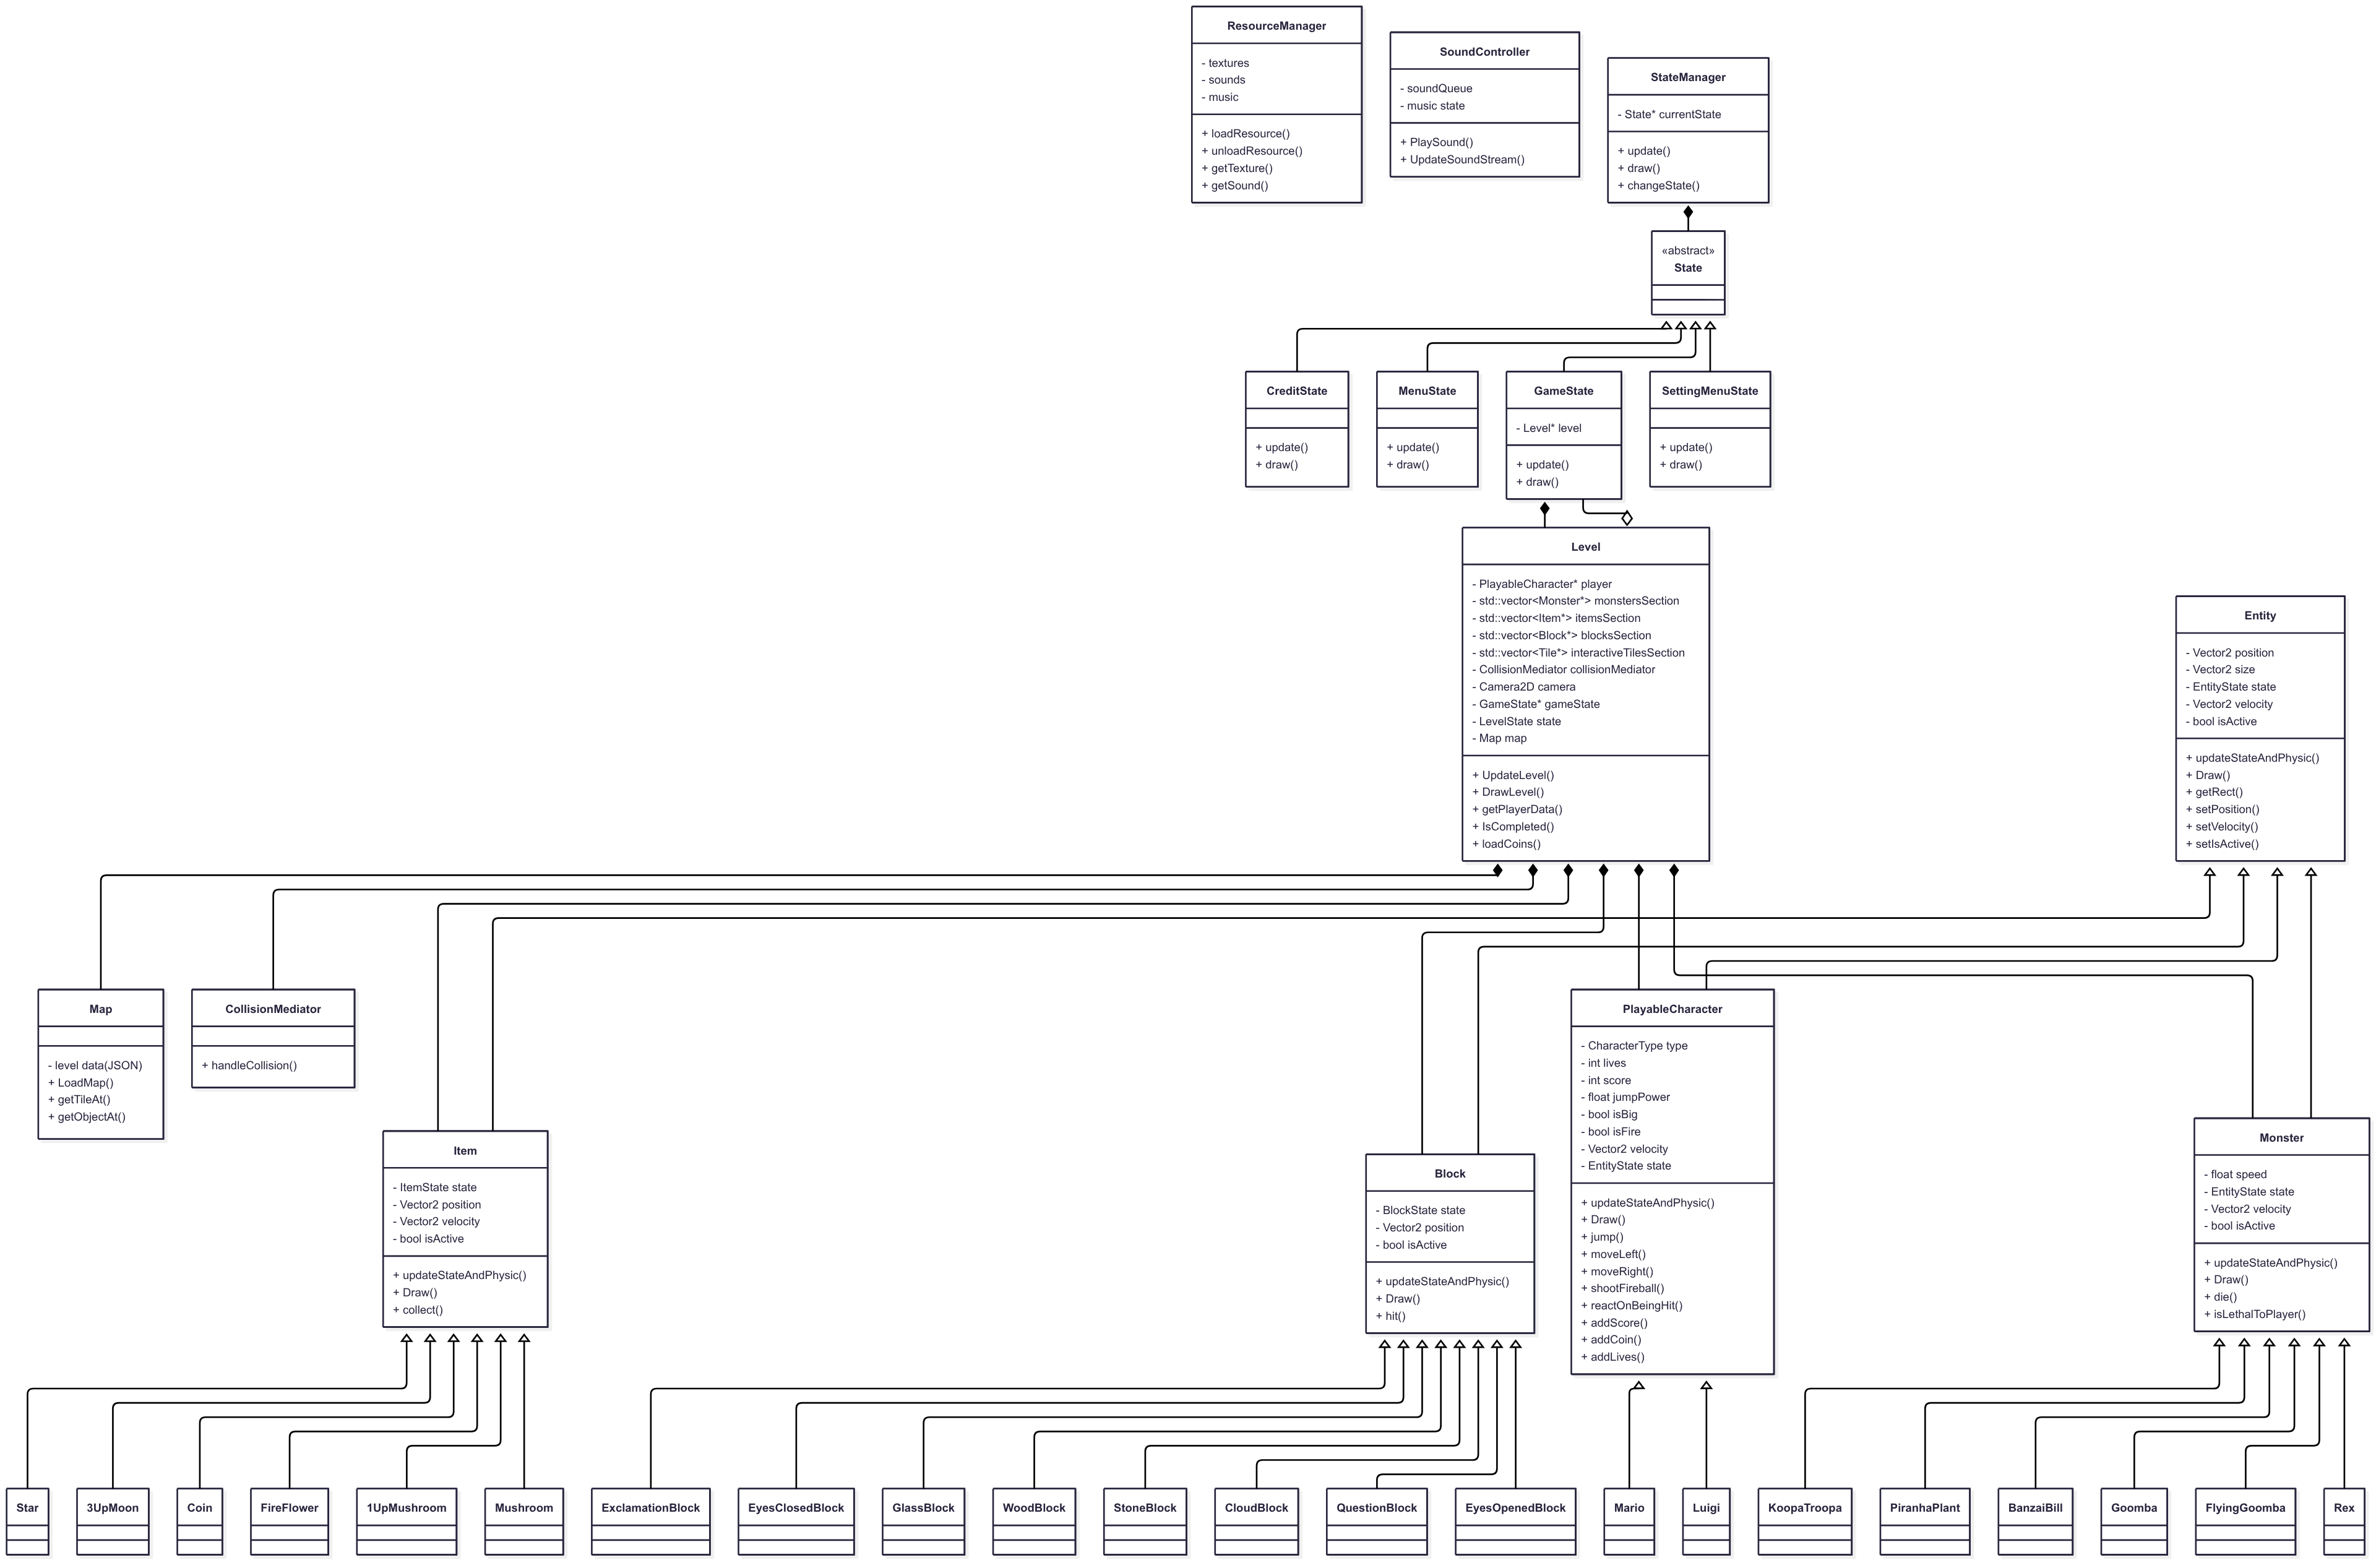
\includegraphics[width=\textwidth]{img/class_diagram}
    \caption{UML Class Diagram of Main Project Architecture}
    \label{fig:uml_diagram}
\end{figure}
               % Tables can follow logic or manual
\clearpage
\section{Code Snippets}

\begin{flushleft}
  This section presents representative code snippets for core mechanics and systems in the Super Mario OOP Project, aligned with the actual implementation logic from the source files.  
\end{flushleft}


\subsection*{Player Jump and Power-Up Collection}
\begin{lstlisting}[language=C++, caption={Mario Jump and Power-Up Collection}]
void PlayableCharacter::jump() {
    if (onGround) {
        velocity.y = -jumpPower;
        onGround = false;
        SoundController::getInstance().PlaySound("smw_jump.wav");
    }
}
void CollisionMediator::HandleMarioWithItem(Mario*& mario, Item*& item, CollisionInfo AtoB) {
    if (AtoB == COLLISION_NONE)
        return;

    if (item && CheckCollisionRecs(mario->getRect(), item->getRect())) {
        if (auto* mushroom = dynamic_cast<Mushroom*>(item)) {
            mushroom->collect();
            mario->setBig(true);
            mario->addScore(1000);
        }
        else if (auto* fireFlower = dynamic_cast<FireFlower*>(item)) {
            fireFlower->collect();
            mario->setFire(true);
            mario->addScore(1000);
        }
    }
}
\end{lstlisting}

\subsection*{Monster Movement and Defeat}
\begin{lstlisting}[language=C++, caption={Goomba Movement and Stomp Defeat}]
void Goomba::updateStateAndPhysic() {
    if (!isActive) return;
    velocity.x = -speed;
    position.x += velocity.x * GameClock::getInstance().DeltaTime;
}
void CollisionMediator::HandleMarioWithMonster(Mario*& mario, Monster*& monster, CollisionInfo AtoB) {
    if (AtoB == COLLISION_SOUTH && mario->getVelocity().y > 0) {
        mario->addScore(400);
        monster->die();
        mario->setVelocity(Vector2{mario->getVelocity().x, -600}); // Bounce
        SoundController::getInstance().PlaySound("smw_stomp.wav");
    } else {
        mario->reactOnBeingHit();
    }
}
\end{lstlisting}

\subsection*{Block Hit and Item Spawn}
\begin{lstlisting}[language=C++, caption={Question Block Hit and Item Spawn}]
void QuestionBlock::hit(Mario* mario) {
    if (state == BlockState::UNUSED) {
        state = BlockState::USED;
        spawnItem();
        SoundController::getInstance().PlaySound("smw_power-up_appears.wav");
    }
}
void QuestionBlock::spawnItem() {
    if (containsMushroom) {
        auto* mushroom = new Mushroom(position + Vector2{0, -size.y});
        Level::getInstance().addItem(mushroom);
    }
}
\end{lstlisting}

\subsection*{Level Update Loop}
\begin{lstlisting}[language=C++, caption={Level Update and Collision Handling}]
void Level::UpdateLevel() {
    player->updateStateAndPhysic();
    for (auto& section : monstersSection)
        for (auto* monster : section)
            monster->updateStateAndPhysic();
    for (auto& section : itemsSection)
        for (auto* item : section)
            item->updateStateAndPhysic();
    for (auto& section : blocksSection)
        for (auto* block : section)
            block->updateStateAndPhysic();

    // Collision checks
    collisionMediator.handleCollisions(player, monstersSection, itemsSection, blocksSection);
}
\end{lstlisting}

\subsection*{Resource Management (Singleton Pattern)}
\begin{lstlisting}[language=C++, caption={ResourceManager Singleton Usage}]
Texture2D& ResourceManager::getTexture(const std::string& name) {
    if (textures.count(name) == 0) {
        textures[name] = LoadTexture(("resources/Entity/" + name).c_str());
    }
    return textures[name];
}
void ResourceManager::unloadResource() {
    for (auto& pair : textures) {
        UnloadTexture(pair.second);
    }
    textures.clear();
}
\end{lstlisting}        % Code after context

\input{content/figures.tex}              % Screenshots at the end (visual)

\clearpage
\section*{References}
\addcontentsline{toc}{section}{References}

\begin{itemize}
  \item Visualization Demo. (2024, Apr 1). \textit{Interactive Data Structures Visualizer using C++ and raylib} [Video]. YouTube. \url{https://www.youtube.com/watch?v=UiZGTIYld1M}
  \item raylib Setup with vcpkg for Visual Studio. (n.d.). GitHub Wiki. \url{https://github.com/raysan5/raylib/wiki/Working-on-Windows#visual-studio-vcpkg}
  \item RayMario Demo. (2020, Sep 20). \textit{Mario-like Game implemented with raylib in C++} [Video]. YouTube. \url{https://youtu.be/pq5NuXYhXYo}
  \item Buzatto, D. (n.d.). \textit{RayMario – A Super Mario-like clone using raylib and C++}. GitHub repository. \url{https://github.com/davidbuzatto/RayMario}
  \item Refactoring.Guru. (n.d.). \textit{Design Patterns}. \url{https://refactoring.guru/design-patterns}
  \item Viblo. (n.d.). \textit{Design Patterns Overview}. Viblo Community. \url{https://viblo.asia/s/design-patterns-68Z00n2NZkG}
  \item Wikipedia contributors. (n.d.). \textit{Behavior tree (artificial intelligence, robotics and control)}. In Wikipedia. \url{https://en.wikipedia.org/wiki/Behavior_tree_(artificial_intelligence,_robotics_and_control)}
\end{itemize}

%Conclusion
\section{Conclusion}
\begin{flushleft}

The Super Mario OOP Project demonstrates how object-oriented programming and modular design can be used to recreate a classic platformer game in C++. By separating game logic into clear classes and using patterns like singletons and state management, we achieved both functional gameplay and maintainable code.

\vspace{1em}

Despite challenges with timing, collision, and resource handling, our team collaborated effectively to solve problems and deliver a smooth, feature-rich experience. The project structure also makes it easy to add new features or expand the game in the future.

\vspace{1em}

Overall, this project provided valuable experience in C++ development, teamwork, and game architecture, and serves as a strong foundation for future enhancements
% Appendix – separate page
\clearpage
\appendix

\section*{Appendix: Repository and Video}
\begin{itemize}
    \item GitHub Repository: \url{https://github.com/letongthiennha/Mario}
    \item Demo Video (YouTube): 
\end{itemize}
\end{flushleft}
\end{document}